\documentclass[nologo,a4paper,12pt]{article}

\usepackage[T1]{fontenc}
\usepackage[utf8]{inputenc}
\usepackage{lmodern}
\usepackage{microtype}
\usepackage[left=2.3cm,right=2.3cm,top=2.35cm,bottom=2.35cm,headheight=25pt]{geometry}
\usepackage{xcolor}
\usepackage{fancyhdr}
\usepackage{titlesec}
\usepackage{mdframed}
\usepackage{amssymb}
\usepackage{booktabs}
\usepackage{tabularx}
\usepackage{array}
\usepackage{parskip}
\usepackage{enumitem}
\usepackage{graphicx}
\usepackage{subcaption}
\usepackage{float}
\usepackage{seqsplit}
\usepackage{tikz}
\usetikzlibrary{arrows.meta,positioning}
\usepackage{hyperref}
\usepackage[capitalize]{cleveref}

\definecolor{mls@blue}{RGB}{0,83,134}
\definecolor{mls@gray}{RGB}{100,100,100}
\definecolor{mls@lightgray}{RGB}{245,245,245}
\definecolor{mls@green}{RGB}{40,130,60}
\definecolor{mls@lightgreen}{RGB}{220,245,225}
\definecolor{mls@red}{RGB}{160,30,30}
\definecolor{mls@lightyellow}{RGB}{255,252,220}
\definecolor{mls@yellow}{RGB}{180,140,0}

\hypersetup{colorlinks=true,linkcolor=mls@blue,urlcolor=mls@blue}
\pagestyle{fancy}
\fancyhf{}
\fancyhead[L]{\small\color{mls@gray}Introduction to Machine Learning Safety}
\fancyhead[R]{\small\color{mls@gray}Safety Case Report}
\fancyfoot[C]{\small\color{mls@gray}\thepage}
\renewcommand{\headrulewidth}{0.6pt}
\renewcommand{\headrule}{{\color{mls@blue}\rule{\headwidth}{0.6pt}}}

\titleformat{\section}{\large\bfseries\color{mls@blue}}{\thesection.\ }{0.4em}{}[{
  \color{mls@blue}\titlerule[0.6pt]}]
\titlespacing{\section}{0pt}{1.4em}{0.45em}
\titleformat{\subsection}{\normalsize\bfseries}{}{0em}{}
\titlespacing{\subsection}{0pt}{1.0em}{0.35em}
\setlist{nosep,leftmargin=1.6em}
\setcounter{tocdepth}{1}
\newcolumntype{Y}{>{\raggedright\arraybackslash}X}

\mdfdefinestyle{claimstyle}{backgroundcolor=mls@lightgray,linecolor=mls@blue,
  linewidth=2pt,topline=false,rightline=false,bottomline=false,
  innerleftmargin=12pt,innerrightmargin=10pt,innertopmargin=7pt,
  innerbottommargin=7pt,skipabove=0.5em,skipbelow=0.5em}
\mdfdefinestyle{subclaim}{backgroundcolor=white,linecolor=mls@blue,
  linewidth=0.8pt,roundcorner=3pt,innerleftmargin=9pt,innerrightmargin=9pt,
  innertopmargin=5pt,innerbottommargin=5pt,skipabove=0.6em,skipbelow=0.45em,
  nobreak=true}
\mdfdefinestyle{evidencestyle}{backgroundcolor=mls@lightgreen!30,
  linecolor=mls@green,linewidth=0.8pt,roundcorner=3pt,
  innerleftmargin=9pt,innerrightmargin=9pt,innertopmargin=5pt,
  innerbottommargin=5pt,skipabove=0.55em,skipbelow=0.45em,nobreak=true}

\newcommand{\verdictmet}{\textbf{\color{mls@green}$\checkmark$~Met}}
\newcommand{\verdictnotmet}{\textbf{\color{mls@red}$\times$~Not met}}
\newcommand{\verdictpartial}{\textbf{\color{mls@yellow}$\approx$~Partial}}

\begin{document}

\begin{titlepage}
\thispagestyle{empty}
\centering
\vspace*{2.1cm}
{
\color{mls@blue}\rule{\linewidth}{2pt}}\\[1.2em]
{\color{mls@blue}\Huge\bfseries Final Report}\\[0.8em]
{\LARGE Introduction to Machine Learning Safety}\\[0.6em]
{\large\color{mls@gray}CARLA Autonomous Driving Perception System}\\[1.2em]
{\color{mls@blue}\rule{\linewidth}{2pt}}

\vspace{2.6cm}
\begin{tabularx}{\linewidth}{@{}l X@{}}
  \textbf{Student:} & Gopeshkumar Harsukh Rabadiya \\[1.0em]
  \textbf{Matriculation number:} & 261637 \\[1.0em]
  \textbf{Date:} & 19 August 2026 \\[1.0em]
  \textbf{Code repository:} &
  \href{https://github.com/gopesh-007/carla-ml-safety-baseline}{
  \texttt{gopesh-007/carla-ml-safety-baseline}} \\
\end{tabularx}

\vfill
{\color{mls@gray}\small Otto-von-Guericke University Magdeburg}
\end{titlepage}

\clearpage
\tableofcontents

\clearpage
\section{System Description}
\label{sec:system-description}

\subsection{Provided system description}

An autonomous vehicle (AV) prototype operates in an urban environment. The system is
composed of the following components:

\begin{enumerate}
  \item \textbf{Camera:} A single forward-facing RGB camera, rigidly mounted behind the windshield, provides images at 10\,Hz. There are \emph{no other perception sensors} (no radar, no LiDAR, no ultrasonic).
  \item \textbf{Perception models:} Three separate binary classifiers each receive the camera frame and output one binary prediction: \emph{pedestrian present}, \emph{vehicle present}, or \emph{traffic light present}. Each model was trained exclusively on sunny daytime data collected in the CARLA simulator.
  \item \textbf{Distance oracle:} A separate model estimates the distance to detected pedestrians and
    vehicles. You may assume this model is perfect for the sake of this course.
  \item \textbf{Planning module:} The rule-based planner consumes the three perception outputs together with the current vehicle speed and steering angle. Its primary safety-relevant decisions are whether to continue driving, request deceleration, or issue an emergency brake command. Emergency braking is triggered when the pedestrian detector reports a pedestrian within a critical distance, when the vehicle detector indicates a road user ahead within a speed-dependent
    threshold, or when the traffic-light detector indicates that stopping is required at an approaching intersection. The planner does not have access to raw camera images and relies entirely on the perception models' outputs.
  \item \textbf{Vehicle actuators:} Throttle, brake, and steering commands are executed by drive-by-wire actuators. Emergency braking applies maximum deceleration within the physical limits of the vehicle.
  \item \textbf{Human safety operator:} A trained operator sits in the driver seat and monitors the road. The operator can override the autopilot at any time by pressing the brake pedal or turning the steering wheel. The operator receives a visual dashboard showing the current perception output and system status, but no auditory alerts are provided. During testing, operators work 4-hour shifts.
  \item \textbf{Operating environment:} The vehicle is tested on public urban roads at speeds up to 50\,km/h. The intended conditions are daytime, dry weather, and mapped intersections. However, weather and lighting conditions can change during a test drive (e.g.\ sudden cloud cover, low sun angle, rain onset).
\end{enumerate}

\subsection{Key design limitations (by construction)}

\begin{itemize}
  \item No sensor redundancy --- a single camera is the only perception input.
  \item No other safety mechanisms are deployed yet.
  \item The human operator is the only fallback if the automation fails.
  \item The operator may exhibit a non-zero probability of delayed or missed intervention, especially under prolonged monitoring.
\end{itemize}

The traffic-light detector reports only the presence of a traffic light, not its state (red / green). The planner therefore cannot, on its own, decide whether to stop at a signalized intersection. This is a limitation of the system as specified that no model metric can close, so it is recorded as a known design limitation in \cref{sec:residual}.

\subsection{Architecture \& training}

All three classifiers use the same ResNet-18 architecture, initialized from scratch without
pretrained weights, with the final layer replaced by one logit. Images are resized to
$224\times224$, converted to tensors, and no data augmentation or pretrained normalization is
applied. A sigmoid and threshold of 0.5 are used for evaluation.

For each classification task, the dataset contains 7,200 training, 3,600 validation and 3,600
test frames. Training uses Adam ($10^{-3}$), batch size 32, weighted binary cross-entropy, and
five epochs. The positive-class weights were pedestrian $5482/1718$ and traffic light
$1924/5276$. The evaluated vehicle
checkpoint accidentally reused the pedestrian weight $5482/1718$, although its class counts are
5,458 positive and 1,742 negative. I retained this historical configuration to keep the published
checkpoint reproducible and treat it as a training defect rather than silently changing the
experiment. Training was performed on CPU. Code, result files and exact checkpoint hashes are
listed in Appendix~\ref{app:reproducibility}.

\clearpage
\section{Operational Design Domain}
\label{sec:odd}

The intended ODD is a narrow subset of the provided system's stated environment. ``Detection''
below distinguishes a required runtime check from what is currently implemented.

{\footnotesize
\begin{tabularx}{\linewidth}{@{}p{1.8cm}YYY@{}}
\toprule
\textbf{Dimension} & \textbf{Operating conditions} & \textbf{Non-operating conditions} & \textbf{Detection / status} \\
\midrule
Weather & Dry; clear or partly cloudy; no precipitation & Fog, rain, snow, spray or severe glare & Image/OOD monitor required; k-NN evaluated offline only \\
Lighting & Daylight with usable contrast & Night, dusk, tunnel or direct low-sun glare & Image-quality/OOD check required; not integrated \\
Camera & Fixed forward RGB; clean, unblocked, 10\,Hz & Blocked, damaged, blurred or missing/late frames & Heartbeat and quality monitor required; absent \\
Scene type & Mapped urban roads and intersections similar to source town & Unmapped town, highway, unusual road geometry & Map/geofence plus OOD monitor required; absent \\
Speed & $0$--$50$\,km/h, forward travel & Above 50\,km/h or reverse automation & Vehicle-state check available to planner \\
\bottomrule
\end{tabularx}}

\subsection{ODD gap analysis}

Training covers only sunny daytime images from one source domain. It does not cover fog, rain,
night, alternative towns, camera faults, glare, or combinations of these factors. The supplied
test variants add fog/day/source-town, rain/night/source-town and dry/day/Town-01. These are useful
stress tests, but they do not make those conditions part of the validated ODD. In particular,
there is no evidence for night in Town-01, fog in Town-01, rainy daylight, or physical camera
faults. Performance claims are therefore limited to the standard dry/day/source-town test split.

\subsection{ODD coverage}

The reproducible $k$-projection calculation uses three recorded context factors: weather,
lighting and town. All individual values occur, but their combinations are sparse.

\begin{mdframed}[style=evidencestyle]
\textbf{Evidence ($k$-projection coverage):}
\begin{center}
\begin{tabular}{cccc}
\toprule
$k$ & Observed & Possible & Coverage \\
\midrule
1 & 7 & 7 & 100.0\% \\
2 & 10 & 16 & 62.5\% \\
3 & 4 & 12 & 33.3\% \\
\bottomrule
\end{tabular}
\end{center}
\end{mdframed}

Coverage falls sharply as interactions are considered. Consequently, passing a one-factor test
cannot justify performance on combined shifts. Uncovered combinations remain unverified residual
risk rather than being interpolated from the four observed scenarios.

\subsection{ODD violation response}

The required response is: flag the violation, suppress normal ``continue'' control, begin a
controlled deceleration, issue an unmistakable operator alert, and reach a minimal-risk stop if
the operator does not take over within a verified bound. The submitted prototype only evaluates
OOD detection offline. It has no integrated OOD signal, automatic minimal-risk manoeuvre,
auditory alert, or measured takeover bound. This gap is captured by SC-5, SC-7 and SC-9,
evaluated through V-4 and V-5.

\clearpage
\section{Safety Analysis (STPA)}
\label{sec:stpa}

\subsection{Control structure}

\begin{figure}[ht]
\centering
\resizebox{0.98\linewidth}{!}{%
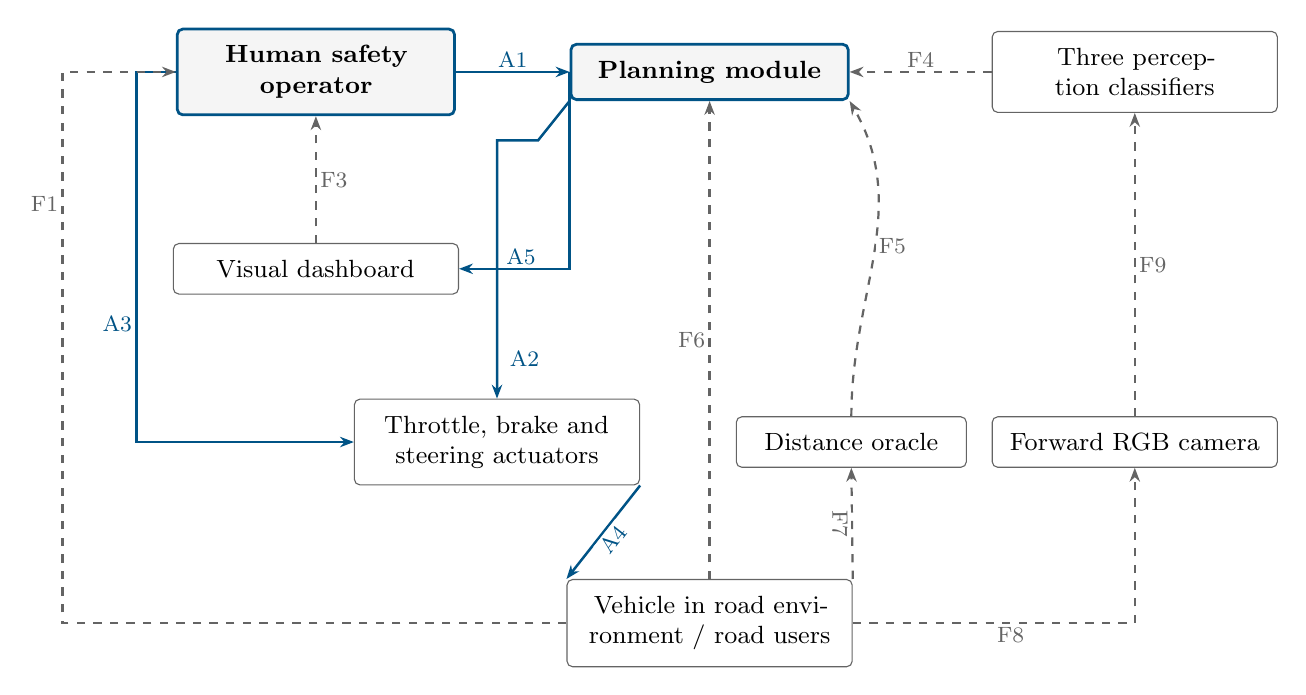
\begin{tikzpicture}[
  ctrl/.style={rectangle,rounded corners=2pt,draw=mls@blue,fill=mls@lightgray,
    line width=1pt,text width=3.1cm,align=center,font=\small\bfseries,inner sep=6pt},
  proc/.style={rectangle,rounded corners=2pt,draw=mls@gray,fill=white,
    text width=3.2cm,align=center,font=\small,inner sep=6pt},
  act/.style={-{Stealth[length=5pt]},mls@blue,line width=0.9pt},
  feed/.style={-{Stealth[length=5pt]},mls@gray,dashed,line width=0.8pt},
  elabel/.style={fill=white,fill opacity=.92,text opacity=1,inner sep=1.2pt},
  every node/.style={font=\footnotesize}
]
\node[ctrl] (op) at (-5.0,3.0) {Human safety operator};
\node[ctrl] (plan) at (0,3.0) {Planning module};
\node[proc] (per) at (5.4,3.0) {Three perception classifiers};
\node[proc] (dash) at (-5.0,0.5) {Visual dashboard};
\node[proc] (actu) at (-2.7,-1.7) {Throttle, brake and steering actuators};
\node[proc,text width=2.5cm] (dist) at (1.8,-1.7) {Distance oracle};
\node[proc] (cam) at (5.4,-1.7) {Forward RGB camera};
\node[proc] (road) at (0,-4.0) {Vehicle in road environment / road users};

\draw[act] (op.east) -- node[elabel,above]{A1} (plan.west);
\draw[act] (plan.south west) -- ++(-0.4,-0.5) -| (actu.north);
\node[elabel,text=mls@blue] at (-2.35,-0.65) {A2};
\draw[act] (op.west) -- ++(-0.5,0) |- node[elabel,pos=.34,left]{A3} (actu.west);
\draw[act] (actu.south east) -- node[elabel,below,sloped]{A4} (road.north west);
\draw[act] (plan.west) |- node[elabel,pos=.72,above]{A5} (dash.east);

\draw[feed] (road.west) -- ++(-6.4,0) |- node[elabel,pos=.38,left]{F1} (op.west);
\draw[feed] (dash.north) -- node[elabel,right]{F3} (op.south);
\draw[feed] (per.west) -- node[elabel,above]{F4} (plan.east);
\draw[feed] (dist.north) to[out=90,in=300] node[elabel,pos=.52,right]{F5} (plan.south east);
\draw[feed] (road.north) -- node[elabel,left]{F6} (plan.south);
\draw[feed] (road.north east) -- node[elabel,below,sloped]{F7} (dist.south);
\draw[feed] (road.east) -| node[elabel,pos=.28,below]{F8} (cam.south);
\draw[feed] (cam.north) -- node[elabel,right]{F9} (per.south);
\end{tikzpicture}}
\caption{Safety control structure. Solid blue arrows are control actions; dashed grey arrows are feedback.}
\label{fig:control-structure}
\end{figure}

{\footnotesize A1 engage/disengage; A2 continue/decelerate/emergency brake; A3 operator brake/steer
override; A4 actuator commands; A5 dashboard status/alert command. F1 direct road view; F3
dashboard display; F4 binary labels; F5 oracle distance; F6 speed/steering; F7 true distance;
F8 road scene; F9 camera frames.}

The solid arrows distinguish the two control paths. The planning module is the automated
controller and issues driving commands through A2, while the human operator controls engagement
through A1 and can bypass the planner through the direct override path A3. The actuators translate
these commands into physical vehicle motion through A4. The planner also issues dashboard status
and takeover alerts through A5.

The dashed arrows close the feedback loops. The planner receives binary perception outputs,
oracle distance, speed and steering information through F4--F6. Camera images originate from the
road environment through F8 and F9, while the operator receives both a direct view of the road
through F1 and the dashboard display through F3.

In STPA, a control action is not inherently unsafe; it becomes unsafe in a particular context. A
continue command is normally valid, but becomes unsafe when a pedestrian is within stopping
distance, the traffic-light state is unknown, or the vehicle has left its ODD. The planner cannot
inspect the image that produced a label, and the operator can override the actuators but receives
no auditory alert. These limitations motivate the unsafe control actions below.

\subsection{Losses and system hazards}

{\small
\begin{tabularx}{\linewidth}{@{}p{0.8cm}p{4.6cm}Y@{}}
\toprule
\textbf{ID} & \textbf{Loss} & \textbf{Why unacceptable} \\
\midrule
L-1 & Death or serious injury to occupants or other road users & Irreversible harm to people \\
L-2 & Damage to vehicles, property or infrastructure & Physical and economic harm \\
L-3 & Traffic-law violation & Endangers road users and invalidates road approval \\
L-4 & Loss of availability or traffic continuity & Unnecessary stops can obstruct traffic or provoke rear-end conflict \\
\bottomrule
\end{tabularx}

\vspace{0.6em}
\begin{tabularx}{\linewidth}{@{}p{0.8cm}Yp{2.5cm}@{}}
\toprule
\textbf{ID} & \textbf{Hazardous system state} & \textbf{Loss(es)} \\
\midrule
H-1 & Vehicle moves without adequate braking while a pedestrian or vehicle is within stopping distance & L-1, L-2 \\
H-2 & Vehicle continues into a signalised intersection without reliable stop/state information & L-1, L-2, L-3 \\
H-3 & Automation remains active outside its ODD or with degraded camera input & L-1--L-4 \\
H-4 & Planner acts on an incorrect, overconfident perception output without timely override & L-1, L-2 \\
H-5 & Vehicle brakes unnecessarily or for too long when no road user requires it & L-1, L-2, L-4 \\
\bottomrule
\end{tabularx}}

\clearpage
\subsection{Unsafe control actions}

{\scriptsize
\begin{tabularx}{\linewidth}{@{}p{1.0cm}p{1.5cm}p{2.1cm}p{1.6cm}p{1.25cm}Y@{}}
\toprule
\textbf{ID} & \textbf{Controller} & \textbf{Control action} & \textbf{UCA type} & \textbf{Hazard} & \textbf{Context in which unsafe} \\
\midrule
UCA-1 & Planner & Emergency brake & Not provided & H-1,H-4 & An actual road user is within stopping distance and emergency braking is required \\
UCA-2 & Planner & Brake/decelerate & Too late & H-1,H-2 & Action begins after remaining distance is insufficient \\
UCA-3 & Planner & Release brake & Too early & H-1 & Road user remains present but a temporary miss/occlusion occurs \\
UCA-4 & Planner & Continue & Provided & H-2 & Signal state is unknown at an approaching intersection \\
UCA-5 & Planner & Continue & Provided & H-3 & ODD or camera-validity condition has been violated \\
UCA-6 & Planner & Alert/takeover request & Not provided & H-3,H-4 & Perception is invalid, OOD or low-confidence \\
UCA-7 & Operator & Engage/keep automation & Provided & H-3 & Preconditions are outside the declared ODD \\
UCA-8 & Operator & Override & Too late/not provided & H-1--H-4 & Automation fails during prolonged passive monitoring \\
UCA-9 & Planner & Emergency brake & Provided too long & H-5 & False positive occurs while no relevant road user is present \\
\bottomrule
\end{tabularx}}

\subsection{Causal loss scenarios}

{\footnotesize
\begin{tabularx}{\linewidth}{@{}p{1.0cm}p{1.8cm}Y@{}}
\toprule
\textbf{ID} & \textbf{For UCA} & \textbf{Causal scenario} \\
\midrule
LS-1 & 1--3 & In-distribution false negative or unstable frame-wise output suppresses or prematurely releases braking \\
LS-2 & 1--6 & Small adversarial perturbation changes a perception output \\
LS-3 & 1,4--6 & Misclassification is overconfident, so confidence appears safe \\
LS-4 & 5--7 & Fog, night or new-town input is not detected as outside the validated domain \\
LS-5 & 1--3 & Single camera is affected by occlusion, small objects, blur or shortcut features \\
LS-6 & 4 & Traffic-light classifier reports presence but not red/green state \\
LS-7 & 6,8 & No automatic fallback/auditory alert; four-hour monitoring contributes to delayed override \\
LS-8 & 1--3,8 & 10\,Hz acquisition, inference, planning or human response introduces unsafe delay \\
LS-9 & 9 & Vehicle false positive under fog repeatedly requests unnecessary braking \\
LS-10 & 5,7 & ODD boundaries are not enforced before or during operation \\
\bottomrule
\end{tabularx}}

\subsection{Safety constraints}

{\footnotesize
\begin{tabularx}{\linewidth}{@{}p{1.0cm}p{1.5cm}Yp{1.35cm}p{1.3cm}@{}}
\toprule
\textbf{ID} & \textbf{Controls} & \textbf{Safety constraint} & \textbf{Level} & \textbf{Verified} \\
\midrule
SC-1 & LS-1,5 & ID recall shall be $\geq0.90$ pedestrian and $\geq0.85$ traffic light/vehicle & Model & V-1 \\
SC-2 & LS-2 & Recall drop at FGSM $\varepsilon=.05$ shall be $<.10$ & Model & V-2 \\
SC-3 & LS-3 & ECE after validation-only calibration shall be $<.05$ & Model & V-3 \\
SC-4 & LS-4 & OOD monitor shall achieve AUROC $\geq.90$ for each tested model/shift & Model & V-4 \\
SC-5 & LS-3,4,10 & Invalid, OOD or low-confidence input shall suppress ``continue'' and initiate a minimal-risk response & System & V-5 \\
SC-6 & LS-6 & Unknown traffic-light state shall never authorize continue; provide state sensing or default stop & System & V-5 \\
SC-7 & LS-7,8 & Failure shall trigger visual and auditory takeover alert; if no response within a verified bound, stop automatically & System & V-5 \\
SC-8 & LS-1,5,9 & Brake/release shall use temporal confirmation and hysteresis, with false-positive limits & System & V-5 \\
SC-9 & LS-10 & ODD preconditions shall be checked before engagement and continuously enforced & System & V-4,V-5 \\
SC-10 & LS-8 & End-to-end sensing/control latency shall be bounded and braking shall not depend solely on operator reaction & System & V-5 \\
\bottomrule
\end{tabularx}}

\clearpage
\section{Safety Case}
\label{sec:safety-case}

\begin{mdframed}[style=claimstyle]
\textbf{Top claim:} \textit{The CARLA autonomous driving system operates safely within its
Operational Design Domain as specified.}
\end{mdframed}

The claim would require every safety-critical constraint to be supported. The argument below
follows Evidence $\Rightarrow$ V $\Rightarrow$ SC $\Rightarrow$ LS $\Rightarrow$ UCA
$\Rightarrow$ H $\Rightarrow$ L. A failed verification is retained and propagated as residual
risk; it is not reclassified as acceptable.

{\small
\begin{tabularx}{\linewidth}{@{}Yp{2.0cm}p{2.35cm}p{1.7cm}@{}}
\toprule
\textbf{Verification} & \textbf{SC(s)} & \textbf{Loss scenarios} & \textbf{Hazards} \\
\midrule
V-1 ID detection performance & SC-1 & LS-1, LS-5 & H-1,H-2,H-4 \\
V-2 Perturbation robustness & SC-2 & LS-2 & H-1,H-2,H-4 \\
V-3 Calibrated uncertainty & SC-3 & LS-3 & H-1--H-4 \\
V-4 OOD detection & SC-4, SC-9 & LS-4, LS-10 & H-3,H-4 \\
V-5 Safe system fallback & SC-5--SC-10 & LS-3,4,6--10 & H-1--H-5 \\
\bottomrule
\end{tabularx}}

\subsection{V-1: In-distribution detection performance}

\begin{mdframed}[style=subclaim]
\textbf{Constraint:} SC-1 requires sufficient ID recall.\\
\textbf{Metric:} Recall on the 3,600-frame dry/day/source-town test split. Thresholds:
pedestrian $\geq.90$, traffic light $\geq.85$, vehicle $\geq.85$.
\end{mdframed}

\begin{mdframed}[style=evidencestyle]
\centering
\begin{tabular}{lcccc}
\toprule
Model & Accuracy & Recall & Threshold & Result \\
\midrule
Pedestrian & .7058 & .1076 & .90 & \verdictnotmet \\
Traffic light & .9206 & .9358 & .85 & \verdictmet \\
Vehicle & .7875 & .8537 & .85 & \verdictmet \\
\bottomrule
\end{tabular}

\medskip
\textbf{Overall V-1 verdict: \verdictnotmet}
\end{mdframed}

Pedestrian recall is the safety-dominant result: about nine of ten labelled pedestrian-positive
frames are missed. Traffic-light and vehicle recall pass individually, although the vehicle result
is only 0.0037 above threshold and was produced with the documented class-weight error.

\begin{figure}[H]
\centering
\begin{subfigure}[t]{0.27\linewidth}\centering
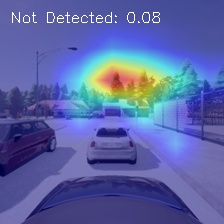
\includegraphics[width=\linewidth]{../outputs/explainability/pedestrian/baseline/gradcam_000780.jpg}
\caption{Dry/day, score .08}\label{fig:grad-day}
\end{subfigure}\hfill
\begin{subfigure}[t]{0.27\linewidth}\centering
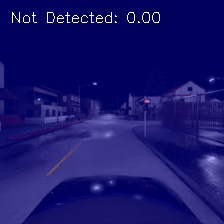
\includegraphics[width=\linewidth]{../outputs/explainability/pedestrian/night/gradcam_001050.jpg}
\caption{Night, score .00}\label{fig:grad-night}
\end{subfigure}\hfill
\begin{subfigure}[t]{0.27\linewidth}\centering
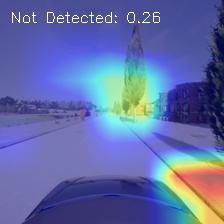
\includegraphics[width=\linewidth]{../outputs/explainability/pedestrian/town01/gradcam_001970.jpg}
\caption{Town-01, score .26}\label{fig:grad-town}
\end{subfigure}
\caption{Pedestrian Grad-CAM examples across conditions.}
\label{fig:gradcam}
\end{figure}

The overlays support, but do not prove, the numerical finding. In \cref{fig:grad-day} the strongest
activation lies in distant foliage/sky rather than a pedestrian silhouette. The selected night
example has no meaningful activation (\cref{fig:grad-night}), while Town-01 produces a strong road-edge/structure
response (\cref{fig:grad-town}). This is consistent with shortcut learning and leaves LS-5 open.

\subsection{V-2: Robustness to input perturbations}

\begin{mdframed}[style=subclaim]
\textbf{Traces to:} SC-2 $\rightarrow$ LS-2 $\rightarrow$ UCA-1/4
$\rightarrow$ H-1/H-2/H-4.\\
\textbf{Metric:} absolute recall drop under untargeted FGSM at $\varepsilon=.05$; required $<.10$.
\end{mdframed}

\begin{mdframed}[style=evidencestyle]
\centering
\begin{tabular}{lcccc}
\toprule
Model & Clean recall & FGSM recall & Drop & Result \\
\midrule
Pedestrian & .1923 & .0000 & .1923 & \verdictnotmet \\
Traffic light & .8987 & .0000 & .8987 & \verdictnotmet \\
Vehicle & .8596 & .0351 & .8246 & \verdictnotmet \\
\bottomrule
\end{tabular}

\medskip
\textbf{Overall V-2 verdict: \verdictnotmet}
\end{mdframed}

The deterministic test uses 100 validation images per model (seed 42), so its clean recalls differ
from V-1. All drops exceed .10 and pedestrian/traffic-light recall reaches zero. This digital test
does not establish a physical attack, but it rejects the stated bound; the non-monotonic vehicle
curve at $\varepsilon=.10$ does not repair failure at the specified .05 point.

\begin{figure}[ht]
\centering
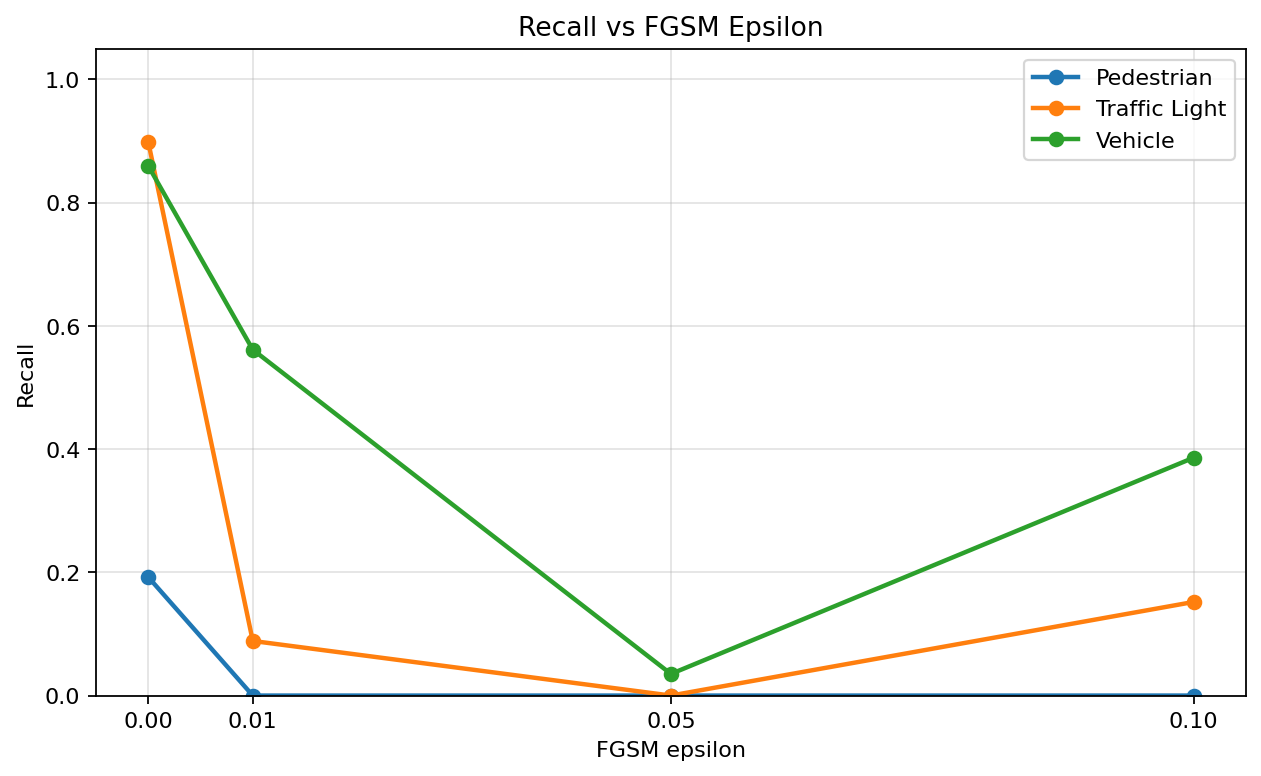
\includegraphics[width=.60\linewidth]{../outputs/adversarial/plots/recall_vs_epsilon.png}
\caption{Recall under the saved FGSM evaluation.}
\label{fig:fgsm}
\end{figure}

\subsection{V-3: Calibrated uncertainty}

\begin{mdframed}[style=subclaim]
\textbf{Traces to:} SC-3 $\rightarrow$ LS-3 $\rightarrow$ UCA-1/4--6
$\rightarrow$ H-1--H-4.\\
\textbf{Metric:} ten-bin ECE on the test set after temperature selection on validation data;
required ECE $<.05$.
\end{mdframed}

\begin{mdframed}[style=evidencestyle]
\centering
\begin{tabular}{lcccc}
\toprule
Model & Temperature & ECE before & ECE after & Result \\
\midrule
Pedestrian & 3.0 & .1477 & .0385 & \verdictmet \\
Traffic light & 1.2 & .0349 & .0246 & \verdictmet \\
Vehicle & 0.9 & .0286 & .0177 & \verdictmet \\
\bottomrule
\end{tabular}

\medskip
\textbf{Overall V-3 verdict: \verdictmet}

\smallskip
Temperature scaling brings all ECE values below .05 without changing class decisions. This
supports SC-3 only on ID data: it neither repairs low recall nor implements SC-5's fallback.
For the pedestrian model, 3.0 was the upper edge of the search grid; it is therefore the best
evaluated value, not evidence that the unconstrained temperature optimum was found.
\end{mdframed}

\subsection{V-4: Out-of-distribution detection}

\begin{mdframed}[style=subclaim]
\textbf{Traces to:} SC-4/SC-9 $\rightarrow$ LS-4/LS-10 $\rightarrow$ UCA-5--7
$\rightarrow$ H-3/H-4.\\
\textbf{Metric:} feature-space $k$-NN ($k=5$) fitted on 1,000 deterministic validation
references and scored on an independent 1,000-image dry/day test ID subset against 1,000 OOD
images per comparison; required AUROC $\geq.90$ for every tested shift.
\end{mdframed}

\begin{mdframed}[style=evidencestyle]
\centering
\begin{tabular}{lccccc}
\toprule
Model & Fog & Night & Town-01 & Minimum & Result \\
\midrule
Pedestrian & .7794 & 1.0000 & .5168 & .5168 & \verdictpartial \\
Traffic light & .6304 & 1.0000 & .6449 & .6304 & \verdictpartial \\
Vehicle & .9473 & .9875 & .4311 & .4311 & \verdictpartial \\
\bottomrule
\end{tabular}

\medskip
\textbf{Overall V-4 verdict: \verdictpartial}
\end{mdframed}

All three models pass the threshold for night, only the vehicle model passes for fog, and none
passes for Town-01. The detector is therefore not reliable enough to justify accepting either
fog or a new town. Moreover, the evaluated monitor is an offline experiment and is not connected
to the planner. The evidence only partially supports SC-4 and does not satisfy SC-9's continuous
enforcement.

\subsection{V-5: Safe system fallback}

\begin{mdframed}[style=subclaim]
\textbf{Traces to:} SC-5--SC-10 $\rightarrow$ LS-3,4,6--10 $\rightarrow$
UCA-1--9 $\rightarrow$ H-1--H-5.\\
\textbf{Required design:} detected OOD/invalid/low-confidence input causes controlled deceleration,
clear takeover request and automatic minimal-risk stop within verified time bounds.
\end{mdframed}

\begin{mdframed}[style=evidencestyle]
The current design has maximum braking for detected close objects and permits direct human brake
or steering override. However, it has no integrated OOD/confidence response, no camera-health
monitor, no auditory warning, no verified operator takeover time, and no automatic minimal-risk
stop if the operator fails to respond. The presence-only traffic-light output also cannot safely
select continue versus stop.

\medskip
\textbf{Overall V-5 verdict: \verdictnotmet}
\end{mdframed}

Human supervision reduces some risk but is not a bounded fallback, especially during four-hour
monitoring shifts. Since SC-5--SC-10 remain unsatisfied, their associated controls are absent,
and V-1/V-2 already expose frequent model failure, the top claim is \textbf{not supported}.

\clearpage
\section{Residual Risks and Mitigations}
\label{sec:residual}

{\small
\begin{tabularx}{\linewidth}{@{}p{1.0cm}p{1.4cm}YY@{}}
\toprule
\textbf{From} & \textbf{Open hazard} & \textbf{Residual risk} & \textbf{Concrete next control} \\
\midrule
V-1 & H-1,H-4 & Pedestrians are frequently missed in nominal conditions & Retrain on balanced/diverse data; use pretrained detector; validate recall and distance-stratified misses \\
Stress test & H-5 & Vehicle fog false positives can produce unnecessary maximum braking & Correct weighting, include fog negatives, limit false-positive rate, use temporal confirmation/hysteresis \\
V-2 & H-1,H-2,H-4 & Small input perturbations can suppress safety detections & Adversarial training, stronger attacks/physical tests, input-integrity monitoring and independent safety channel \\
V-4 & H-3,H-4 & Fog and Town-01 shifts can be accepted by the tested detector; all Town-01 comparisons fail & Redesign and tune on held-out ID/OOD data; test more towns and combined conditions; integrate monitor with fail-safe action \\
V-5 & H-1--H-5 & Human-only fallback can be delayed or missed & Add audible/haptic alerts, measured takeover bound and automatic minimal-risk stop \\
ODD coverage & H-3 & Most weather--light--town interactions are untested & Scenario-based sampling for missing 2/3-way combinations before widening the ODD \\
\bottomrule
\end{tabularx}}

\subsection{Known design limitations}

\begin{itemize}
  \item \textbf{Traffic-light semantics (H-2):} the classifier I trained answers ``is there a
  traffic light?'', but that turned out to be the wrong question for planning. Presence alone gives
  no red/green state, so a validated state classifier or infrastructure signal is needed. Until then,
  an unknown state has to default to stop.
  \item \textbf{Single-camera dependence (H-1,H-3,H-4):} the system has exactly one perception
  channel. If the camera is occluded or fails, nothing else can compensate. I would add an independent
  radar/LiDAR channel, together with camera diagnostics that can at least detect a bad input.
  \item \textbf{Classification without localization (H-1,H-5):} a frame-level presence label
  collapses very different situations---for example, a pedestrian waiting at the curb and one already
  crossing---into the same signal. Localisation, tracking and path relevance are required before this
  can serve as a driving perception interface.
  \item \textbf{Offline rather than closed-loop evidence (all hazards):} everything reported here
  was measured on saved frames. It therefore establishes neither 10\,Hz latency nor stopping distance,
  controller stability, operator response time or collision rate. Closed-loop scenario testing is the
  necessary next step, not an optional extension of the analysis.
  \item \textbf{Simulator-to-reality gap (H-3,H-4):} I generated no evidence that performance on
  the supplied simulated images would transfer to real public roads. That gap remains open regardless
  of how the other model metrics turn out.
\end{itemize}

The calibrated pedestrian cost experiment (Appendix~\ref{app:additional-evidence}) shows the trade-off:
lowering its threshold eliminates false negatives in this dataset but produces 2,894 false positives.
This reduces one hazard by aggravating H-5 and cannot replace a redesigned detector.

\clearpage
\subsection{Engineering decisions based on the evidence}

I used the experiments not only to compare model metrics, but also to decide which claims about the
prototype could still be defended. The following decisions were made from the final results.

\textbf{Preserve the evaluated checkpoints.} I did not retrain or replace a checkpoint after seeing
the final metrics. In particular, the evaluated vehicle checkpoint reused the pedestrian class
weight. A corrected training run might improve the result, but it would no longer represent the
experiment completed during the semester. I therefore kept the published checkpoint, documented
the defect and treated corrected retraining as future work.

\textbf{Use safety-relevant metrics rather than the most favourable metric.} For detection
performance, I gave recall priority because a false negative can suppress a required braking
request. The pedestrian model shows why accuracy alone was unsuitable: accuracy was .7058 while
recall was only .1076. The opposite problem appeared for the vehicle model in fog. Its F1 score was
.8725, but it predicted vehicle-positive in 3,599 of 3,600 frames. I therefore did not use a single
favourable aggregate metric to support a safety claim.

\textbf{Keep the ODD narrow.} I did not include fog, night or Town-01 in the validated ODD simply
because they had been evaluated. Pedestrian and traffic-light recall reached zero at night, the
vehicle model missed 1,748 vehicles, and three-way weather--lighting--town coverage was only 33.3\%.
These conditions remain stress tests; the supported performance claim is limited to the exact
dry/day/source-town test condition.

\textbf{Use feature $k$-NN as evidence, not as a deployed safety mechanism.} Feature $k$-NN
improved the pedestrian night comparison from .0000 AUROC with MSP to 1.0000, but that benefit did
not generalise across conditions. Pedestrian fog AUROC was .7794, its Town-01 result was .5168,
and no model passed the Town-01 threshold; only the vehicle model passed fog. I therefore retained
$k$-NN as an experimental monitoring candidate, not as a reliable deployed mechanism or permission
for the vehicle to continue driving.

\textbf{Do not present calibration or threshold reduction as a model repair.} I accepted V-3 as
evidence that the confidence scores became more reliable, not that the underlying detections became
correct. Temperature scaling reduced pedestrian ECE from .1477 to .0385 without changing class
decisions. The calibrated cost-sensitive threshold removed pedestrian false negatives on this test
set but created 2,894 false positives. I therefore rejected threshold reduction as a standalone
deployment solution; retraining, localisation, tracking and temporal decision logic are still
required.

\textbf{Restrict the prototype to research use.} The failed pedestrian recall, adversarial recall
collapse, incomplete Town-01 OOD detection and absent automatic fallback outweighed the successful
calibration result. I therefore restricted the acceptable use to offline analysis, simulation and
controlled closed-course research with a safety driver. This leads directly to the deployment
recommendation below.

\clearpage
\subsection{Experimental validity and evidence boundaries}

The experiments provide enough evidence to decide the stated verification checks, but they do not
cover every condition relevant to vehicle safety. I considered the following limitations when
forming the final recommendation.

\textbf{Frames are not the same as independent driving scenarios.} It is tempting to read ``3,600
test frames'' as a large, statistically robust sample, and I want to resist that interpretation.
Neighbouring CARLA frames may come from the same driving sequence and share scenery, weather and
road users. I therefore report the number as a frame count---not as 3,600 independent safety
scenarios. A proper scenario-level evaluation would need separate runs, defined initial conditions
and outcomes such as collision or successful stopping, none of which this dataset provides.

\textbf{The adversarial result has a narrow scope.} I want to be precise about what V-2 actually
tested: untargeted one-step FGSM on a deterministic sample of 100 validation images per model, with
seed 42. The observed drops are enough to reject the stated bound for this protocol. They do not
tell me how frequently adversarial inputs occur in the real world, or how the models behave under
PGD, adversarial patches, physical attacks, compression artefacts, camera noise or other attacks.
Those are separate questions that this experiment was not designed to answer.

\textbf{Calibration remains conditional on ID data.} I selected temperature on the validation split
and computed ten-bin ECE on the test split so that I was not fitting the temperature to the result I
would later report. That protects the V-3 result, but only within its dry/day/source-town scope. For
the pedestrian model, validation NLL was still decreasing at temperature 3.0, the edge of my search
grid. The reported .0385 is therefore the best value I tested, not proof that I found the unconstrained
optimum. ECE also depends on the chosen bins, and I did not verify calibration for fog, night,
Town-01 or later dataset drift.

\textbf{The OOD and ODD numbers cover selected factors only.} The feature detector used $k=5$,
1,000 validation references, an independent 1,000-image dry/day test subset as ID, and 1,000 images
from each OOD condition. AUROC tells me how well the detector ranks the two groups across a complete
comparison; it does not select a runtime threshold or define what the planner should do after a flag.
The coverage calculation has a similar limitation. I used weather, lighting and town because those
were the factors available in the supplied metadata. Object distance, occlusion, object size, traffic
density, glare, blur and camera contamination are absent. The 33.3\% three-way result therefore
describes the three factors for which I had data, not the complete driving environment.

\textbf{These thresholds are project criteria, not certification limits.} The recall, recall-drop,
ECE and AUROC limits are checks defined for this safety case; I am not presenting them as legal or
industry-wide acceptance criteria. The asymmetry matters in practice: a failure is enough to leave
the linked safety constraint open, whereas a pass supports only the particular metric, dataset and
protocol that I evaluated. It does not generalise beyond that evidence.

These limitations do not remove the negative findings. They restrict the scope of the positive
evidence and prevent a model-level result from being interpreted as proof of closed-loop system
safety.

\clearpage
\section{Deployment Recommendation}
\label{sec:deployment}

\begin{mdframed}[style=subclaim]
\textbf{Recommendation:}\quad
$\square$ Deploy \quad $\square$ Deploy with restrictions \quad
$\boxtimes$ \textbf{Do not deploy on public roads}

\medskip
\textbf{Permitted use:} offline analysis and closed-course/simulation research with a safety driver,
without presenting the prototype as an autonomous safety function.

\medskip
\textbf{Justification:} V-1 fails because pedestrian recall is .1076; V-2 fails for all three
models; V-4 is only partial; and V-5's fallback controls are absent. V-3 shows that confidence can
be calibrated, but calibration does not correct decisions or cause a safe response. The traffic-light
state gap and single-camera architecture remain open regardless of model metrics. Therefore the top
safety claim is not supported within even the narrow stated ODD. Deployment should be reconsidered
only after SC-1--SC-10 are satisfied, the associated controls are implemented, and the complete
set is re-verified in closed-loop tests over substantially improved ODD coverage.
\end{mdframed}

The negative recommendation is not a conclusion that the exercises failed. The submitted system
is a baseline, and the evidence successfully identifies where its safety argument breaks and which
engineering controls are needed before a deployment claim could be made.

\subsection{Project reflection and next priorities}

Looking across the semester, the most useful lesson for me was that a favourable model metric is
not automatically a favourable safety result. The pedestrian model reached .7058 accuracy while
recall was only .1076, and the vehicle model reached .8725 F1 in fog while predicting positive in
3,599 of 3,600 frames. Calibration passed its own verification without changing a classification,
and feature $k$-NN separated night well but failed several fog and Town-01 comparisons without
providing a safe planner response. These results
only became meaningful when they were connected to unsafe control actions and possible losses.

The same distinction applies to the safety mechanisms. Calibration, OOD detection and Grad-CAM
were useful diagnostics, but none of them can reduce risk unless the system reacts appropriately.
An uncertainty or OOD flag that still allows ``continue'' does not close the hazard. The required
chain is detection, a bounded planner response, a clear operator warning and an automatic
minimal-risk stop if takeover does not occur.

If I continued the project, I would work in the following order:

\begin{enumerate}
  \item \textbf{Rebuild the perception baseline:} improve pedestrian detection on nominal data,
  correct the vehicle class weight, and provide traffic-light state rather than presence alone.
  \item \textbf{Implement the missing system response:} add camera-health checks, connect calibrated
  uncertainty and OOD monitoring to the planner, and implement the verified fallback and alert path.
  \item \textbf{Generate closed-loop evidence:} test stopping distance, end-to-end latency, operator
  takeover and the missing weather--lighting--town combinations with predefined acceptance criteria.
\end{enumerate}

Adversarial training, stronger attacks and further explainability work would still be useful, but I
would not prioritise them above failed nominal pedestrian detection and the absent fallback. The main
outcome of this project is therefore not a claim that the prototype is safe, but a clearer account of
the evidence and engineering controls that would be required before that claim could be responsibly
reconsidered.

% -------------------------------------------------------- statement of authorship
\clearpage
\thispagestyle{empty}
\begin{center}
  {\large\bfseries\color{mls@blue}Statement of Authorship}
\end{center}

\medskip
\textbf{AI-use disclosure.} I used OpenAI Codex as a supporting tool for code review and debugging,
organising and cross-checking experimental evidence, and assisting with drafting, revising and
formatting parts of the report in LaTeX. I ran the experiments, verified the reported evidence,
and made the final analytical and safety decisions. All AI-assisted suggestions were critically
reviewed and revised before inclusion.

\medskip
I hereby declare that I have independently written the present work and have not used any sources or aids other than
those stated.

Texts, trains of thought, concepts, graphics, etc.\ from external sources that I have directly or
indirectly adopted in my work I have clearly marked as such and provided with complete references
to the respective source. All other content of this work (text parts, figures, tables, etc.)
without corresponding references originates in the copyright sense from me.

I have exclusively used AI systems whose use was approved by the examiner as an aid.

Excluded from the requirement of identification are orthographic or grammatical corrections,
translations, and improvements to formulations that do not alter meaning.

I am aware that AI-generated texts offer no guarantee for the quality of content and text.
I therefore declare that I have used AI systems only as an aid, that I have listed and marked the
AI-generated content, critically reviewed it, and that my independent contribution predominates in
this work.

I confirm that I have fully understood the content of my work and can represent it independently.

\vspace{2.0cm}
\begin{tabularx}{\linewidth}{@{}X c X@{}}
  \cline{1-1} \cline{3-3}
  \multicolumn{1}{l}{\small Place, Date} & & \multicolumn{1}{l}{\small Signature}
\end{tabularx}

\clearpage
\appendix
\section{Additional Material}

\subsection{Reproducibility record}
\label{app:reproducibility}

The public repository is
\url{https://github.com/gopesh-007/carla-ml-safety-baseline}. Exact evaluated checkpoints are
published in release \texttt{v1.0-model-checkpoints}. SHA-256 values are:

{\footnotesize
\begin{tabularx}{\linewidth}{@{}p{4.4cm}Y@{}}
\toprule
File & SHA-256 \\
\midrule
\path{pedestrian_model.pth} & \texttt{\seqsplit{033e991fed2412c7675aa25aada36194d2505c722636fe2b44d5fe67d8e01e0a}} \\
\path{traffic_light_model.pth} & \texttt{\seqsplit{7a2444f42eb8d20c0d515396945eda35348952ab1d7d06329503562547929650}} \\
\path{vehicle_model.pth} & \texttt{\seqsplit{f6d98f8c1bb08fd7201d0a435c032655932d01b0174a75440827d99992f04d2a}} \\
\path{pedestrian_model_backdoor.pth} & \texttt{\seqsplit{cd13f2d3d266e485b8434a000fea883ded5ce68f6b4fd28f518920b3f126b4bb}} \\
\bottomrule
\end{tabularx}}

The repository file \path{EVIDENCE.md} maps each final verification to its script, checkpoint,
protocol and saved output. Principal evidence files are:
{\footnotesize
\begin{itemize}
  \item \nolinkurl{outputs/adversarial/adversarial_results.csv}
  \item \nolinkurl{outputs/uncertainty/calibration_results.csv}
  \item \nolinkurl{outputs/ood/knn_all_models_results.csv}
  \item \nolinkurl{outputs/odd/odd_k_projection_coverage.csv}
\end{itemize}}
The dataset was supplied for the course and is not redistributed.

\subsection{Evidence provenance}
\label{app:evidence-provenance}

The table below is the compact provenance record for the five final verifications. It distinguishes
saved experimental evidence from V-5, which is a negative design inspection rather than a missing
experiment. Exact commands, checkpoint hashes and supporting artifacts are recorded in
\path{EVIDENCE.md}.

{\scriptsize
\renewcommand{\arraystretch}{1.12}
\begin{tabularx}{\linewidth}{@{}p{.62cm}p{3.45cm}p{3.75cm}Yp{1.65cm}@{}}
\toprule
\textbf{ID} & \textbf{Implementation} & \textbf{Evidence record} & \textbf{Protocol} & \textbf{Verdict} \\
\midrule
V-1
& \path{evaluate_pedestrian.py}; \path{evaluate_traffic_light.py}; \path{evaluate_vehicle.py}
& Evaluator console metrics recorded in the README and Section~4
& Complete dry/day/source-town test split; 3,600 frames per model; threshold .5
& \mbox{\verdictnotmet} \\
\addlinespace[.35em]
V-2
& \path{evaluate_adversarial.py}
& \nolinkurl{outputs/adversarial/adversarial_results.csv}
& Random validation subset; 100 frames per model; seed 42; FGSM $\varepsilon=.05$
& \mbox{\verdictnotmet} \\
\addlinespace[.35em]
V-3
& \path{evaluate_uncertainty.py}
& \nolinkurl{outputs/uncertainty/calibration_results.csv}
& Temperature chosen on validation; ten-bin ECE on all 3,600 test frames
& \mbox{\verdictmet} \\
\addlinespace[.35em]
V-4
& \path{evaluate_ood_knn_all_models.py}
& \nolinkurl{outputs/ood/knn_all_models_results.csv}
& $k=5$; 1,000 validation references; independent 1,000-image test ID and 1,000 OOD images per comparison
& \mbox{\verdictpartial} \\
\addlinespace[.35em]
V-5
& System-description and STPA inspection; no fallback implementation
& Sections~1, 3 and 4; no generated result file
& Required fallback functions checked against the described design
& \mbox{\verdictnotmet} \\
\bottomrule
\end{tabularx}}

The V-1 evaluators predate the structured CSV records, so their terminal results are explicitly
identified as transcribed evidence rather than being represented as a file that does not exist.
The README also retains provisional STPA notation from earlier exercises; the final SC/V identifiers
in this report are authoritative for submission.

\subsection{Adverse-condition performance}

{\small
\begin{tabularx}{\linewidth}{@{}llrrrrY@{}}
\toprule
Model & Condition & Accuracy & Precision & Recall & F1 & Interpretation \\
\midrule
Pedestrian & Fog & -- & -- & .315 & .269 & partial degradation \\
Pedestrian & Night & -- & -- & .000 & .000 & complete miss failure \\
Pedestrian & Town-01 & -- & -- & .277 & .180 & below safe threshold \\
Traffic light & Fog & -- & -- & .000 & .000 & complete miss failure \\
Traffic light & Night & -- & -- & .000 & .000 & complete miss failure \\
Traffic light & Town-01 & -- & -- & .283 & .416 & severe degradation \\
Vehicle & Fog & .7739 & .7738 & 1.0000 & .8725 & 3,599/3,600 frames positive \\
Vehicle & Night & .4517 & .8211 & .3724 & .5124 & 1,748 false negatives \\
Vehicle & Town-01 & .6486 & .6885 & .7516 & .7187 & domain-shift degradation \\
\bottomrule
\end{tabularx}}

For vehicle/fog, the confusion counts are TP 2,785, FP 814, TN 1 and FN 0. The high recall and
F1 therefore hide near-constant positive prediction, illustrating why a single favourable metric
cannot discharge H-5.

\subsection{Additional exercise evidence}
\label{app:additional-evidence}

\textbf{Cost-sensitive pedestrian decision.} With false negatives costed at 100 and false
positives at 1, the uncalibrated .5 threshold produced 630 FN, 429 FP and total loss 63,429.
After temperature scaling, the Bayes threshold $1/(100+1)=.0099$ produced 0 FN and 2,894 FP
(loss 2,894). This is safer with respect to missed pedestrians but operationally unusable without
localisation and temporal logic.

\textbf{Backdoor experiment.} A fixed trigger was applied to 171 of 1,718 positive pedestrian
training frames (10\% of that class, 2.4\% of the complete training split). The backdoored
checkpoint achieved 100\% attack success rate on triggered test inputs. This evidence is not part
of V-2's FGSM threshold, but it supports the broader need for training-data provenance and
integrity checks.

\begin{figure}[ht]
\centering
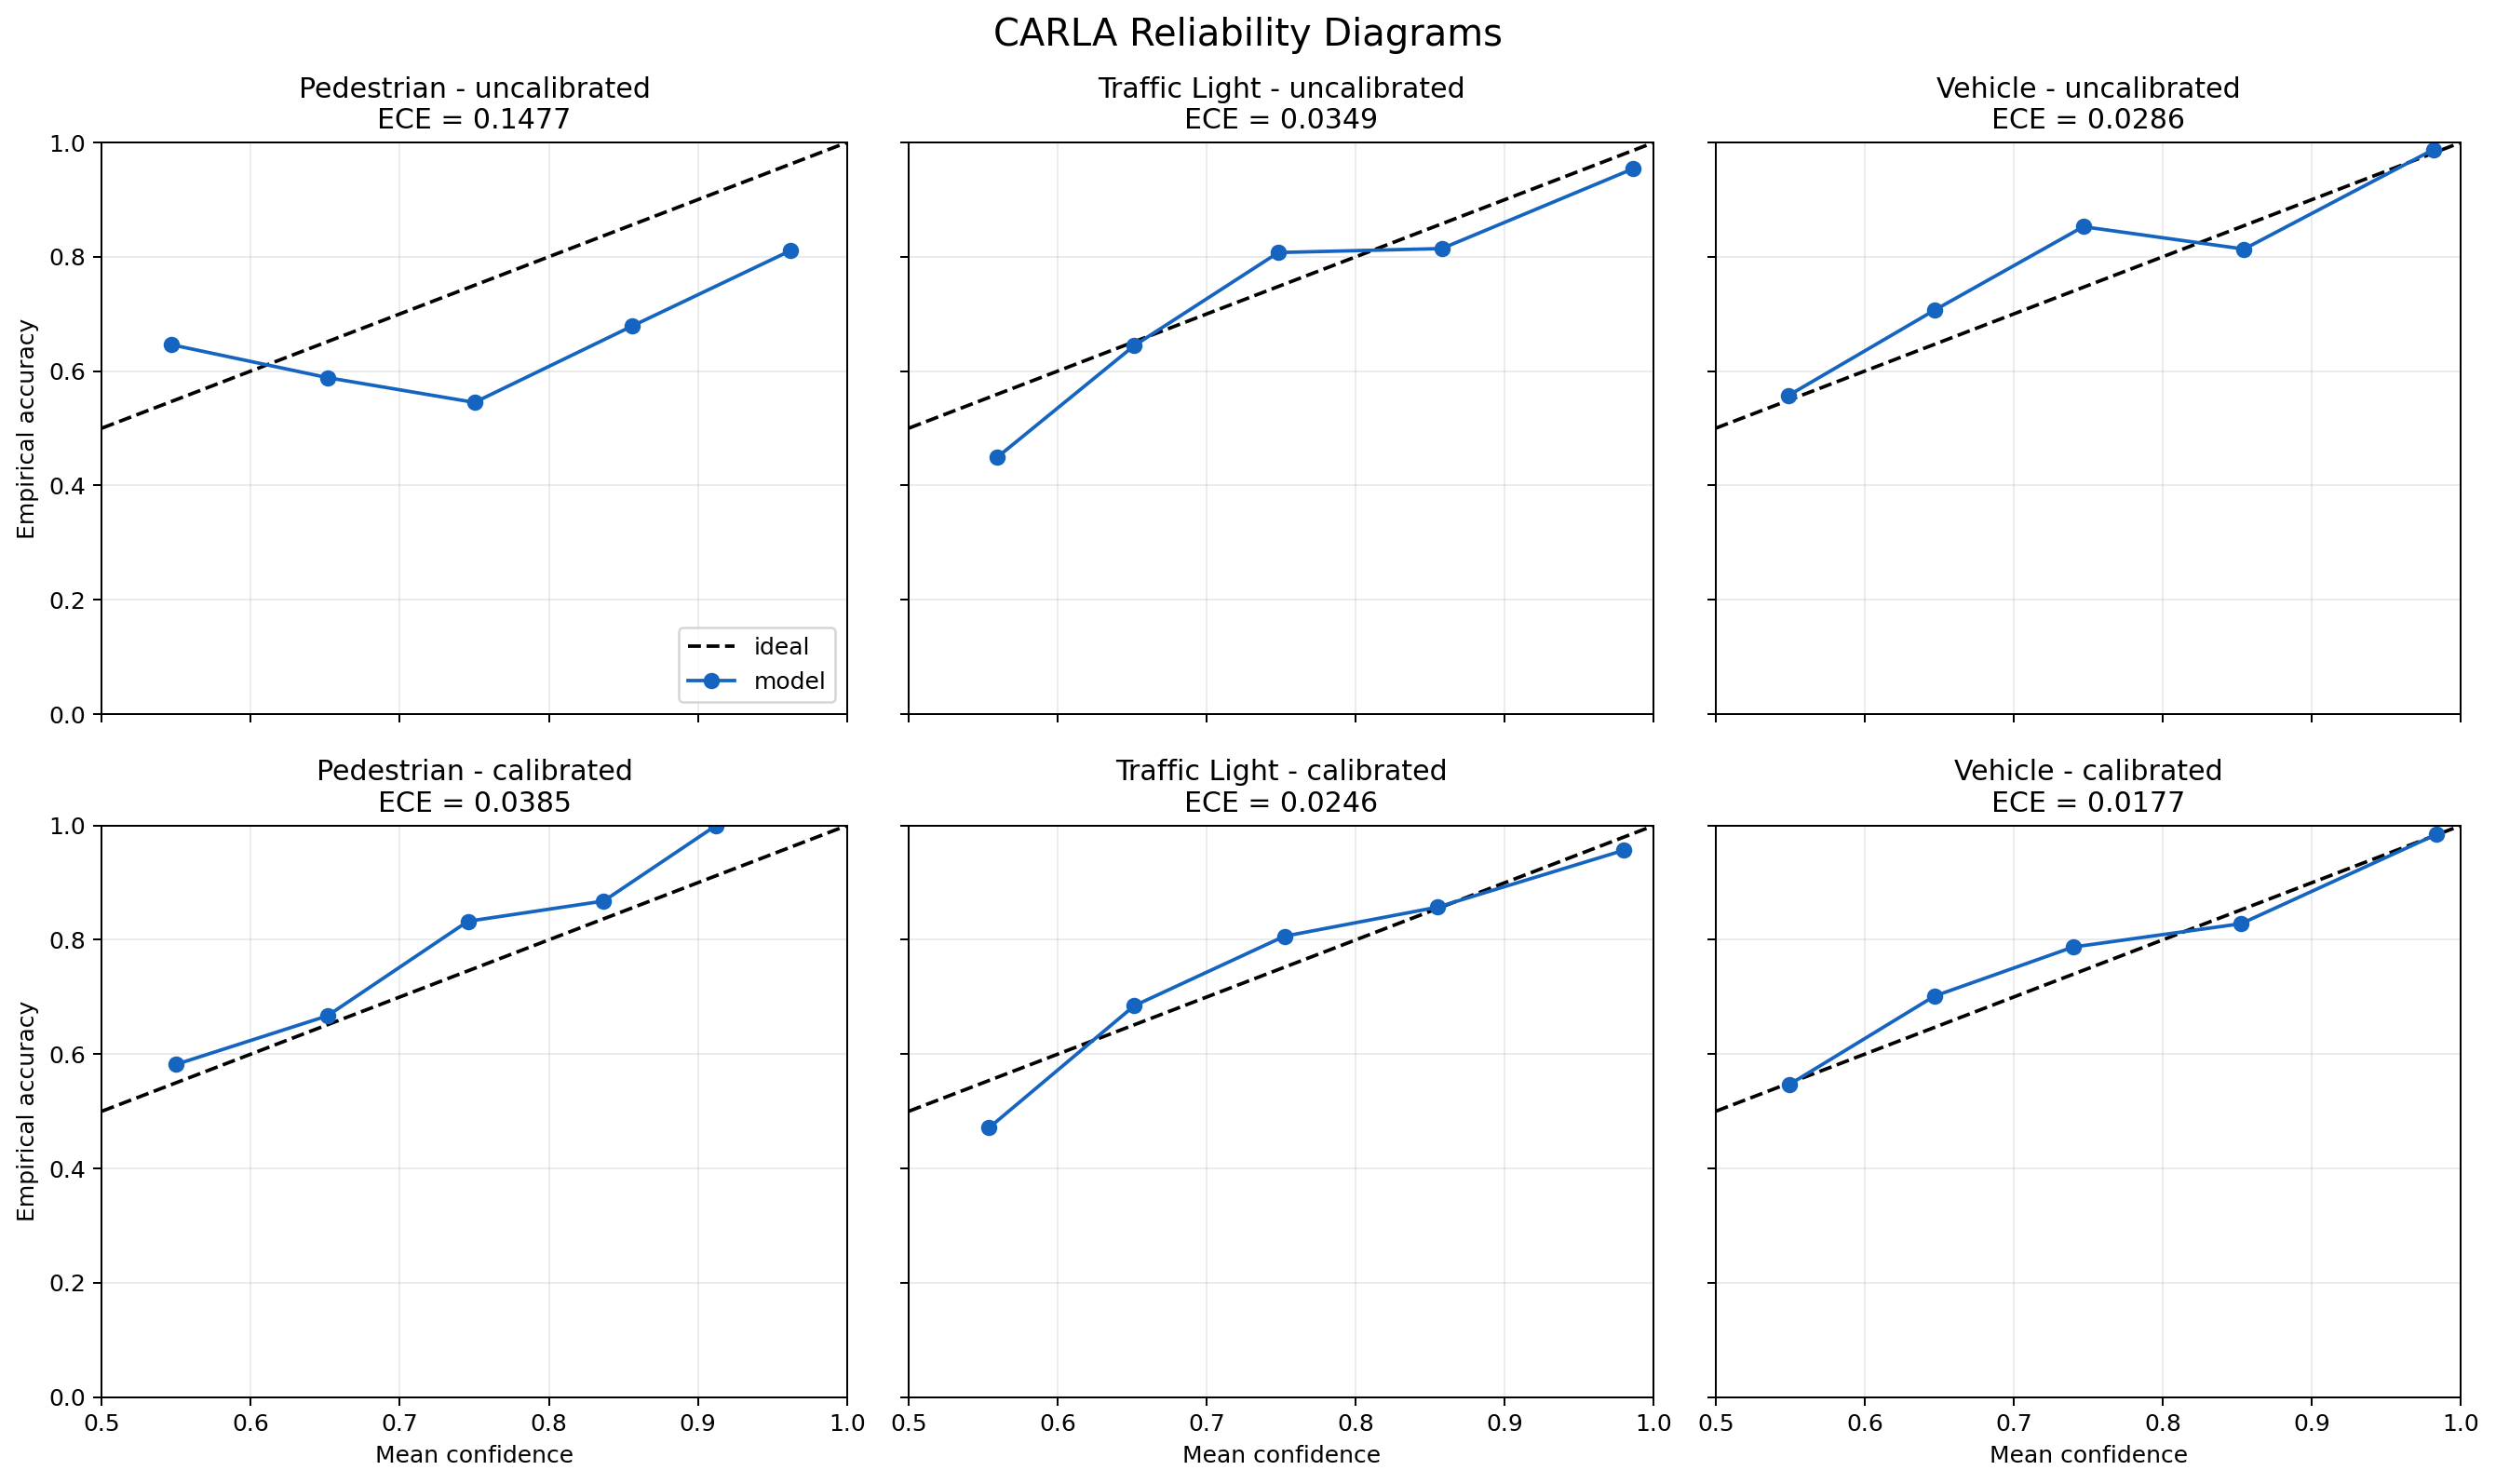
\includegraphics[width=.95\linewidth]{../outputs/uncertainty/reliability_diagrams.png}
\caption{Reliability diagrams before and after temperature scaling.}
\label{fig:reliability}
\end{figure}

\clearpage
\subsection{Evolution of the STPA analysis}
\label{app:stpa-evolution}

The STPA in \cref{sec:stpa} was not written only at the end of the project. I began with the
control structure and loss scenarios from Exercise~2, then updated the analysis whenever a later
experiment exposed a new failure mechanism. The table below records the changes that are supported
by the saved evidence or by assumptions in the final system specification.

{\small
\renewcommand{\arraystretch}{1.08}
\begin{tabularx}{\linewidth}{@{}>{\raggedright\arraybackslash}p{2.55cm}>{\raggedright\arraybackslash}p{5.25cm}Y@{}}
\toprule
\textbf{Stage} & \textbf{Evidence or system assumption} & \textbf{Change made to the STPA} \\
\midrule
Initial Exercise~2 analysis
& The first control structure identified missed braking, operation outside the ODD, unknown
traffic-light state and delayed human intervention as central risks.
& Established the original losses, hazards and UCAs. These remained the basis of the final
analysis rather than being replaced by a separate assessment.\par\smallskip
\textbf{Trace:} L-1--L-4; H-1--H-4; UCA-1--UCA-8 \\
\addlinespace[0.65em]

Adversarial-ML exercise
& At FGSM $\varepsilon=.05$, recall dropped by .1923, .8987 and .8246 for pedestrian,
traffic-light and vehicle models respectively.
& Added adversarial perturbation as a causal explanation for missing or incorrect perception,
together with a measurable robustness constraint.\par\smallskip
\textbf{Trace:} LS-2; SC-2; V-2; H-1,H-2,H-4 \\
\addlinespace[0.65em]

Uncertainty exercise
& The pedestrian model was strongly miscalibrated before scaling (ECE .1477); temperature scaling
reduced it to .0385, but did not change the underlying classifications.
& Added overconfident misclassification as a loss scenario and separated model calibration from
the still-missing system response to low confidence.\par\smallskip
\textbf{Trace:} LS-3; SC-3,SC-5; V-3 \\
\bottomrule
\end{tabularx}}

\clearpage
\subsubsection*{STPA evolution (continued)}

{\small
\renewcommand{\arraystretch}{1.08}
\begin{tabularx}{\linewidth}{@{}>{\raggedright\arraybackslash}p{2.55cm}>{\raggedright\arraybackslash}p{5.25cm}Y@{}}
\toprule
\textbf{Stage} & \textbf{Evidence or system assumption} & \textbf{Change made to the STPA} \\
\midrule

OOD and ODD exercises
& Feature $k$-NN separated night for all models, but only the vehicle model met the fog threshold
and no model met it for Town-01. Three-way ODD coverage was only 33.3\%.
& Added undetected domain shift and unenforced ODD boundaries. Detection and safe response were
kept as separate constraints because the evaluated monitor is offline.\par\smallskip
\textbf{Trace:} LS-4,LS-10; SC-4,SC-9; V-4; H-3,H-4 \\
\addlinespace[0.65em]

Vehicle robustness evaluation
& In fog, 3,599 of 3,600 frames were classified as vehicle-positive, including 814 false
positives.
& Added the possibility of an unnecessary or prolonged braking request and a constraint for
temporal confirmation, hysteresis and false-positive control.\par\smallskip
\textbf{Trace:} H-5; UCA-9; LS-9; SC-8 \\
\addlinespace[0.65em]

Final system specification
& The report specification assumes a perfect distance oracle, while the traffic-light model still
reports presence rather than signal state.
& Removed distance-underestimation as a model failure scenario from the earlier analysis, but
retained the unresolved traffic-light-state scenario and its default-stop constraint.\par\smallskip
\textbf{Trace:} LS-6; UCA-4; SC-6; H-2 \\
\bottomrule
\end{tabularx}}

I did not introduce a new hazard for every experiment. Where possible, later findings were linked
to an existing unsafe control action and expressed as a more specific causal scenario or safety
constraint. This kept the system-level hazard definition stable while allowing the evidence and
mitigations to become more precise over the semester.

\end{document}
